%%%%%%%%%%%%%%%%%%%%%%%%%%%%%%%%%%%%%%%%%
% Masters/Doctoral Thesis 
% LaTeX Template
% Version 2.5 (27/8/17)
%
% This template was downloaded from:
% http://www.LaTeXTemplates.com
%
% Version 2.x major modifications by:
% Vel (vel@latextemplates.com)
%
% This template is based on a template by:
% Steve Gunn (http://users.ecs.soton.ac.uk/srg/softwaretools/document/templates/)
% Sunil Patel (http://www.sunilpatel.co.uk/thesis-template/)
%
% Template license:
% CC BY-NC-SA 3.0 (http://creativecommons.org/licenses/by-nc-sa/3.0/)
%
%%%%%%%%%%%%%%%%%%%%%%%%%%%%%%%%%%%%%%%%%

%----------------------------------------------------------------------------------------
%	PACKAGES AND OTHER DOCUMENT CONFIGURATIONS
%----------------------------------------------------------------------------------------
\documentclass[
11pt, % The default document font size, options: 10pt, 11pt, 12pt
%oneside, % Two side (alternating margins) for binding by default, uncomment to switch to one side
english, % ngerman for German
singlespacing, % Single line spacing, alternatives: onehalfspacing or doublespacing
%draft, % Uncomment to enable draft mode (no pictures, no links, overfull hboxes indicated)
%nolistspacing, % If the document is onehalfspacing or doublespacing, uncomment this to set spacing in lists to single
%liststotoc, % Uncomment to add the list of figures/tables/etc to the table of contents
%toctotoc, % Uncomment to add the main table of contents to the table of contents
%parskip, % Uncomment to add space between paragraphs
%nohyperref, % Uncomment to not load the hyperref package
headsepline, % Uncomment to get a line under the header
chapterinoneline, % Uncomment to place the chapter title next to the number on one line
%consistentlayout, % Uncomment to change the layout of the declaration, abstract and acknowledgements pages to match the default layout
]{MastersDoctoralThesis} % The class file specifying the document structure

\usepackage[utf8]{inputenc} % Required for inputting international characters
\usepackage[T1]{fontenc} % Output font encoding for international characters
\usepackage{mathpazo} % Use the Palatino font by default
\usepackage{cite}

%\usepackage[backend=bibtex,style=numeric,sorting=none, maxbibnames=99]{biblatex} % Use the bibtex backend with the authoryear citation style (which resembles APA)

%\addbibresource{~/BibTex/BibTex.bib} % The filename of the bibliography

\usepackage[autostyle=true]{csquotes} % Required to generate language-dependent quotes in the bibliography

\usepackage{amstext, amsfonts, amsmath, amsbsy, amssymb}
\usepackage{tikz}

%----------------------------------------------------------------------------------------
%	MARGIN SETTINGS
%----------------------------------------------------------------------------------------

\geometry{
	paper=a4paper, % Change to letterpaper for US letter
	inner=2.5cm, % Inner margin
	outer=3.8cm, % Outer margin
	bindingoffset=.5cm, % Binding offset
	top=1.5cm, % Top margin
	bottom=1.5cm, % Bottom margin
	%showframe, % Uncomment to show how the type block is set on the page
}

%----------------------------------------------------------------------------------------
%	THESIS INFORMATION
%----------------------------------------------------------------------------------------

\thesistitle{Anticipating the chemical compositions of organisms across the tree of life.} % Your thesis title, this is used in the title and abstract, print it elsewhere with \ttitle
\supervisor{Prof. Daniel \textsc{Wegmann} \\ \& Dr. Pierre-Marie \textsc{Allard}} % Your supervisor's name, this is used in the title page, print it elsewhere with \supname
\examiner{} % Your examiner's name, this is not currently used anywhere in the template, print it elsewhere with \examname
\degree{Master of Science in Bioinformatics and Computational Biology} % Your degree name, this is used in the title page and abstract, print it elsewhere with \degreename
\author{Marco \textsc{Visani}} % Your name, this is used in the title page and abstract, print it elsewhere with \authorname
\addresses{} % Your address, this is not currently used anywhere in the template, print it elsewhere with \addressname

\subject{Biological Sciences} % Your subject area, this is not currently used anywhere in the template, print it elsewhere with \subjectname
\keywords{} % Keywords for your thesis, this is not currently used anywhere in the template, print it elsewhere with \keywordnames
\university{\href{https://www.unifr.ch/}{University of Fribourg}} % Your university's name and URL, this is used in the title page and abstract, print it elsewhere with \univname
\department{\href{https://www.unifr.ch/bio/en/}{Department of Biology}} % Your department's name and URL, this is used in the title page and abstract, print it elsewhere with \deptname
\group{\href{https://www.unifr.ch/bio/en/groups/wegmann/}{Wegmann Group} \& \href{https://www.unifr.ch/bio/en/groups/allard/}{COMMONS Lab}} % Your research group's name and URL, this is used in the title page, print it elsewhere with \groupname
\faculty{\href{https://www.unifr.ch/scimed/en/}{Faculty of Science and Medicine}} % Your faculty's name and URL, this is used in the title page and abstract, print it elsewhere with \facname

\AtBeginDocument{
\hypersetup{pdftitle=\ttitle} % Set the PDF's title to your title
\hypersetup{pdfauthor=\authorname} % Set the PDF's author to your name
\hypersetup{pdfkeywords=\keywordnames} % Set the PDF's keywords to your keywords
}


%----------------------------------------------------------------------------------------
%	MATH STUFF
\usepackage{amstext, amsfonts, amsmath, amsbsy, amssymb}
\DeclareMathOperator{\Poisson}{Poisson}
\DeclareMathOperator{\Multinom}{Multinom}
\DeclareMathOperator{\logit}{logit}
\DeclareMathOperator{\cov}{cov}
\DeclareMathOperator{\Ind}{I}
\def\P{\mathbb{P}}
\def\E{\mathbb{E}}

\def\x{\boldsymbol{x}}

\def\btau{\boldsymbol{\tau}}
\def\bmu{\boldsymbol{\mu}}
\def\bxi{\boldsymbol{\xi}}
\def\bLambda{\boldsymbol{\Lambda}}
\def\bP{\boldsymbol{P}}



\def\Ccal{{\cal C}}
\def\E{{\cal E}}
\def\I{{\cal I}}
\def\N{{\cal N}}
\def\M{{\cal M}}
\def\R{{\cal R}}
\def\T{{\cal T}}
\def\X{{\cal X}}
\def\Y{{\cal Y}}
\def\Z{{\cal Z}}

%----------------------------------------------------------------------------------------

\linespread{1.25}
\begin{document}


\frontmatter % Use roman page numbering style (i, ii, iii, iv...) for the pre-content pages

\pagestyle{plain} % Default to the plain heading style until the thesis style is called for the body content

%----------------------------------------------------------------------------------------
%	TITLE PAGE
%----------------------------------------------------------------------------------------

\begin{titlepage}
\begin{center}

\vspace*{.06\textheight}
{\scshape\LARGE \univname\par}\vspace{1.5cm} % University name
\textsc{\Large Master Thesis}\\[0.5cm] % Thesis type

\HRule \\[0.4cm] % Horizontal line
{\huge \bfseries \ttitle\par}\vspace{0.4cm} % Thesis title
\HRule \\[1.5cm] % Horizontal line
 
\begin{minipage}[t]{0.4\textwidth}
\begin{flushleft} \large
\emph{Author:}\\
\href{mailto:contact@vismarco.ch}{\authorname} % Author name - remove the \href bracket to remove the link
\end{flushleft}
\end{minipage}
\begin{minipage}[t]{0.4\textwidth}
\begin{flushright} \large
\emph{Supervisors:} \\
\href{mailto:daniel.wegmann@unifr.ch}{Prof. Daniel \textsc{Wegmann}} \\
\href{mailto:pierre-marie.allard@unifr.ch}{Dr. Pierre-Marie \textsc{Allard}}% Supervisor name - remove the \href bracket to remove the link  
\end{flushright}
\end{minipage}\\[3cm]
 
\vfill

\large \textit{A thesis submitted in fulfillment of the requirements \\ for the degree of \degreename}\\[0.3cm] % University requirement text
\textit{in the}\\[0.4cm]
\groupname\\\deptname\\[2cm] % Research group name and department name
 
\vfill

{\large \today}\\[4cm] % Date
%\includegraphics{Logo} % University/department logo - uncomment to place it
 
\vfill
\end{center}
\end{titlepage}

%----------------------------------------------------------------------------------------
%	DECLARATION PAGE
%----------------------------------------------------------------------------------------

\begin{declaration}
\addchaptertocentry{\authorshipname} % Add the declaration to the table of contents
\noindent I, \authorname, declare that this thesis titled, \enquote{\ttitle} and the work presented in it are my own. I confirm that:

\begin{itemize} 
\item This work was done wholly or mainly while in candidature for a research degree at this University.
\item Where any part of this thesis has previously been submitted for a degree or any other qualification at this University or any other institution, this has been clearly stated.
\item Where I have consulted the published work of others, this is always clearly attributed.
\item Where I have quoted from the work of others, the source is always given. With the exception of such quotations, this thesis is entirely my own work.
\item I have acknowledged all main sources of help.
\item Where the thesis is based on work done by myself jointly with others, I have made clear exactly what was done by others and what I have contributed myself.\\
\end{itemize}
 
\noindent Signed:\\
\rule[0.5em]{25em}{0.5pt} % This prints a line for the signature
 
\noindent Date:\\
\rule[0.5em]{25em}{0.5pt} % This prints a line to write the date
\end{declaration}

\cleardoublepage

%----------------------------------------------------------------------------------------
%	QUOTATION PAGE
%----------------------------------------------------------------------------------------

\vspace*{0.2\textheight}

\noindent\enquote{\itshape Thanks to my solid academic training, today I can write hundreds of words on virtually any topic without possessing a shred of information, which is how I got a good job in journalism.}\bigbreak

\hfill Dave Barry

%----------------------------------------------------------------------------------------
%	ABSTRACT PAGE
%----------------------------------------------------------------------------------------

\begin{abstract}\label{sec:abstract}
\addchaptertocentry{\abstractname} % Add the abstract to the table of contents
The Thesis Abstract is written here (and usually kept to just this page). The page is kept centered vertically so can expand into the blank space above the title too\ldots
\end{abstract}

%----------------------------------------------------------------------------------------
%	ACKNOWLEDGEMENTS
%----------------------------------------------------------------------------------------

\begin{acknowledgements}\label{sec:acknowledgements}
\addchaptertocentry{\acknowledgementname} % Add the acknowledgements to the table of contents
The acknowledgments and the people to thank go here, don't forget to include your project advisor\ldots
\end{acknowledgements}

%----------------------------------------------------------------------------------------
%	LIST OF CONTENTS/FIGURES/TABLES PAGES
%----------------------------------------------------------------------------------------

\tableofcontents % Prints the main table of contents

\listoffigures % Prints the list of figures

\listoftables % Prints the list of tables

%----------------------------------------------------------------------------------------
%	ABBREVIATIONS
%----------------------------------------------------------------------------------------

\begin{abbreviations}{ll}\label{sec:abbreviations} % Include a list of abbreviations (a table of two columns)

\textbf{LAH} & \textbf{L}ist \textbf{A}bbreviations \textbf{H}ere\\
\textbf{WSF} & \textbf{W}hat (it) \textbf{S}tands \textbf{F}or\\

\end{abbreviations}

%----------------------------------------------------------------------------------------
%	PHYSICAL CONSTANTS/OTHER DEFINITIONS
%----------------------------------------------------------------------------------------

%\begin{constants}{lr@{${}={}$}l} % The list of physical constants is a three column table
%
%% The \SI{}{} command is provided by the siunitx package, see its documentation for instructions on how to use it
%
%Speed of Light & $c_{0}$ & \SI{2.99792458e8}{\meter\per\second} (exact)\\
%%Constant Name & $Symbol$ & $Constant Value$ with units\\
%
%\end{constants}

%----------------------------------------------------------------------------------------
%	SYMBOLS
%----------------------------------------------------------------------------------------

\begin{symbols}{lll}\label{sec:symbols} % Include a list of Symbols (a three column table)

$a$ & distance & \si{\meter} \\
$P$ & power & \si{\watt} (\si{\joule\per\second}) \\
%Symbol & Name & Unit \\

\addlinespace % Gap to separate the Roman symbols from the Greek

$\omega$ & angular frequency & \si{\radian} \\

\end{symbols}

%----------------------------------------------------------------------------------------
%	DEDICATION
%----------------------------------------------------------------------------------------

%\dedicatory{For/Dedicated to/To my\ldots} 

%----------------------------------------------------------------------------------------
%	THESIS CONTENT - CHAPTERS
%----------------------------------------------------------------------------------------

\mainmatter % Begin numeric (1,2,3...) page numbering

\pagestyle{thesis} % Return the page headers back to the "thesis" style

% Include the chapters of the thesis as separate files from the Chapters folder
% Uncomment the lines as you write the chapters

%\include{Chapters/1_introduction}
%\include{Chapters/2_litterature_review} 
%\include{Chapters/3_methods}
%\include{Chapters/4_results} 
%\include{Chapters/5_discussion} 
%\include{Chapters/6_conclusion}

\chapter{Introduction}\label{chap:intro}

\section{Natural Products: Definition and Roles}\label{sec:NP def and roles}
Natural Products (NPs) are chemical entities biosynthesized by living organisms \cite{AllNatural2007}. Many NPs are metabolites, which can be positioned along a specialization gradient from core metabolites, fulfilling essential functions and found in a wide range of organisms, to specialized metabolites, much more restricted across the tree of life. Natural Products research is a transdisciplinary field with interests spanning from fundamental structural aspects of naturally occurring molecular entities to their effects on living organisms and extending to the study of chemically mediated interactions within entire ecosystems. We will use \textit{Rutz et al.}'s in \cite{rutzLOTUSInitiativeOpen2022} definition of Natural Product \textit{as any chemical entity found in a living organism}, \textit{i.e.} a structure-organism pair. This pair holds an additional and fundamental element - a reference to the experimental evidence establishing the linkage between the chemical structure and the biological organism

\section{The Importance of Natural Products in Therapeutics and Ecosystem Functioning}
Unique in their chemical structures and functionalities, specialized metabolites serve as the cornerstone of today's therapeutic applications. Their relevance extends beyond human and veterinary medicine, touching on areas such as agriculture, the food industry, cosmetics, and an array of other sectors. Intrinsically linked to renewable resources, these natural products hold substantial value within the circular economy concept.

The intricacies of their biological roles and structural characterization are crucial to fully grasp the functioning of ecosystems. These complexities influence a myriad of aspects, from the impact on individual organisms to the overall chemically mediated interactions within entire ecosystems. Despite their multifaceted nature, which presents significant challenges at the molecular level - particularly due to their powerful biological activities (privileged structures) and intricate synthetic accessibility the role of these metabolites is indispensable.

Natural products have also contributed to the development of many foundational scientific concepts, including but not limited to stereochemistry, optical activity, regioselectivity, and chirality. Their diverse and complex nature continually inspires researchers, sparking the creation of innovative tools that can mimic natural processes to control bioregulation mechanisms and address practical challenges \cite{drasarGrowingImportanceNatural2019}.

Even though they're complex and challenging to describe, the role of natural products in therapeutic uses and ecosystem functionality cannot be overstated. Current developments aim to unlock this potential more efficiently, emphasizing the ongoing advancements across all sectors associated with natural products.

\section{The LOTUS Database and Current Efforts}
In recent years, efforts have been made to anticipate metabolic networks or occurrences of molecules in selected taxa. A significant resource is the LOTUS database \cite{rutzLOTUSInitiativeOpen2022} developed and maintained by the \href{https://www.unifr.ch/bio/en/groups/allard/}{COMMONS lab}, which currently lists over 750'000 occurrences of natural products. Despite this, no model has been proposed to predict their occurrence across the tree of life. The LOTUS initiative aims to address these shortcomings by consolidating and sharing structure-organism pair information via an open platform, providing transformative potential for natural products research and beyond. This process involves the harmonization, curation, validation, and open dissemination of referenced structure-organism pairs. Furthermore, LOTUS data's embedding into the vast Wikidata knowledge graph facilitates new biological and chemical insights. The contemporary bioinformatic capabilities offered by the LOTUS initiative have the potential to reshape knowledge management, analysis, and interpretation of data in natural products research.

\section{Project Description and Objectives}
The goal of this project is to develop such a model and to train it using large-scale metabolomics and other occurrence data.

%\chapter{Literature Review}


\chapter{Methodology}
\section{Random Markov Field}\label{sec:methods:random markov field}
We seek to infer the presence or absence of metabolites in a group of samples compartmentalized by several discrete dimensions such as e.g. species, tissue or environmental conditions. We assume that the pattern of presence and absence of these metabolites is modulated by similarities within each dimensions. For instance, closely related species may share a similar set of metabolites and  metabolites related in their synthesis may share a similar distribution across species. To model such similarities, we adopt a Markov Random Field approach \cite{sherringtonSolvableModelSpinGlass1975, kindermannMarkovRandomFields1980}.

Let $D$ denote the total number of dimensions, of which, without loss of generality, the first shall be the metabolite. Each dimension $d=1, \ldots, D$ consist of a set $\E_d$ of discrete entries (e.g. individual species along the species dimension). We model similarities between the entries of dimension $d$ using a Markov process along a known tree $\T_d$ consisting of $\N_d = \E_d \cup \R_d \cup \I_d$ nodes, of which the entries $\E_d$ are leaves, connected to the set of roots $\R_d$ through a set $\I_d$ of internal nodes; $\E_d \cap \R_d = \varnothing$, $\E_d \cap \I_d = \varnothing$ and $\R_d \cap \I_d = \varnothing$. For every node $n \in \N_d, n \notin \R_d$ that is not a root, let $p(n) \in \N_d$ denote its parent node and $b(n) \geq 0$ the length of the branch connecting it to its parent.

Let $\X$ denote a Markov Random Field of which each variable $x \in \X$ represents a combination of nodes from each of the $D$ dimensions and indicates the presence($x=1$) or absence ($x=0$) of metabolite for that combination of nodes. Let $\delta_d(x) \in \N_d$ reflect the node of $x$ in dimension $d$ with $\delta_1(x)$ indicating the metabolite of $x$, and let $\delta(x)=(\delta_1(x), \ldots, \delta_D(x))$. We only consider two sets of variables: 1) the set $\Y$ of variables representing an entry in each dimension such that for a variable $y\in\Y$, $\delta_d(y) \in \E_d$ for all $d=1, \ldots, D$, and 2) the set $\Z$ of variables representing leaves in all dimensions except one such that for a variable $z \in \Z$, $\delta_k(z) \in \I_k$ and $\delta_d(z) \in \E_d$ for all $d \neq k$. We then have $\X = \Y \cup \Z$ and $\Y \cap \Z = \varnothing$.

We suppose that the joint density of $\X$ can be factorized over a set of cliques $\Ccal$. Each clique $c \in \Ccal$ consist of a set of variables $x_1, x_2, \ldots \in \X$ that represent the same leaves in all but one dimension $k$. Specifically, for all $x \in c$, $\delta_d(x) \in \E_d$ for all $d \neq k$ and $\delta_k(x) \in \N_k$, and for all $x_i, x_j \in c$, $\delta_{-k}(x_i) = \delta_{-k}(x_j)$, where $\delta_{-k}(x)$ denotes the vector of nodes of $x$ in all dimensions but $k$. For such a clique, we will refer to the dimension $\nu(c) = k$ as its \emph{variable} dimension and will denote by $\delta_{-\nu(c)}(c)$ the vector of nodes in the \emph{fixed} dimensions. By definition, $\delta_{-\nu(c)}(c)=\delta_{-\nu(c)}(x)$ for every $x \in c$.

We will further denote by $\Ccal_k \subset \Ccal$ the subset of cliques that share the variable dimension $k$, i.e. $\nu(c)=k$ for all $c \in \Ccal_k$. Note that each clique is in exactly one subset ($\Ccal_k \cap \Ccal_d = \varnothing$ for all $k \neq d$) and cliques of the same subset do not share any variables ($c_1 \cap c_2 = \varnothing$ for all $c_1, c_2 \in C_k$). However, each variable $x \in \Y$ will be part of exactly one clique from each subset: the clique $c \in \Ccal_k$ for which $\delta_{-k}(c) = \delta_{-k}(x)$. In contrast, each variable $x \in \Z$ will be part of exactly one clique: the clique $c \in \Ccal$ for which $\delta_{-\nu(c)}(c) = \delta_{-\nu(c)}(x)$ and $\delta_{\nu(c)}(x) \in \I_{\nu(c)}$.

The joint density of $\X$ factorizes as
\begin{equation}
	\P(\X) = \prod_{d=1}^D \prod_{c \in \Ccal_d} \phi(c),
\end{equation}

where
we model the clique functions $\phi(c)$ using a Markov model along tree $\T_d$. Let

\begin{equation}
	\bLambda_c =
	\begin{pmatrix}
		-\mu_{c1} & \mu_{c1}\\
		\mu_{c0} & -\mu_{c0}\\
	\end{pmatrix}
\end{equation}

be the rate matrix for changes between states 0 and 1 along the tree. For each node $n \in \N_d, n \notin \R_d$ that is not a root, the transition probabilities between parent node $p(n)$ and $n$ are then given by

\begin{equation}
	\bP(n) = \exp(\bLambda_c b(n)).
\end{equation}

We assume the root state probabilities are given by the stationary distribution of the Markov chain:
\begin{equation}
	\bP_{\infty} = \left(\frac{\mu_{c0}}{\mu_{c0} + \mu_{c1}}, \frac{\mu_{c1}}{\mu_{c0} + \mu_{c1}}\right).
\end{equation}


The clique function $\phi(c)$
\begin{equation}
	\phi(c) = \prod_{x \in c, }\Big( \Ind(x \in \R_{\nu(c)})[\bP_{\infty}]_x + \Ind(x \notin \R_{\nu(c)}) [\bP(\delta_{\nu(c)}(x))]_{p_{c}(x), x} \Big)
\end{equation}

where we used the shorthand $x \in \R_{\nu(c)}$ for $\delta_{\nu(c)}(x) \in \R_{\nu(c)}$ to indicate whether the node in the variable dimension of $c$ of $x$ is a root and $p_{c}(x)$ to identify the variable $z \in c$ for which $\delta_{\nu(c)}(z) = p(\delta_{\nu(c)}(x))$.

\begin{figure}
	\centering
	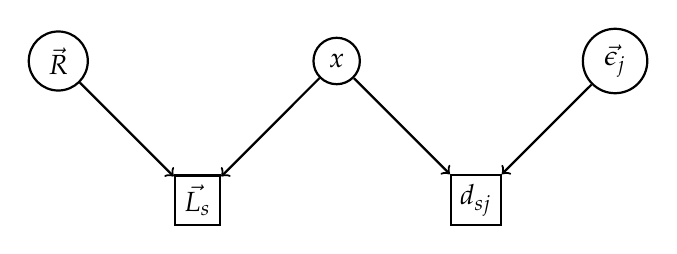
\begin{tikzpicture}[node distance={25mm}, thick, main/.style = {draw, circle}]
		\node[main] (1) {$\boldmath{x}$};
		\node[draw] (4) [below right of=1] {$d_{sj}$};
		\node[draw] (5) [below left of=1] {$\vec{L_s}$};
		\node[main] (6) [above right of=4] {$\vec{\epsilon_j}$};
		\node[main] (7) [above left of=5] {$\vec{R}$};
		
		\draw[->] (1) -- (4);
		\draw[->] (1) -- (5);
		\draw[->] (6) -- (4);
		\draw[->] (7) -- (5);
	\end{tikzpicture}
	\caption{Potential DAG of the model.}
	\label{fig:DAG_model}
\end{figure}

\section{Graph Convolution Neural Network (GraphSAGE)}\label{sec:methods:HinSAGE}
GraphSAGE \cite{hamiltonInductiveRepresentationLearning2017} is an inductive method for learning representations of nodes in graph-structured data. The objective of GraphSAGE is to generate a low-dimensional vector representation for each node in a graph that concisely encapsulates the node's structural and feature information. The central contribution of this method is its capacity for inductive learning, allowing for the generation of embeddings for unseen nodes or even entire unseen graphs, based on the trained model, contrasting it from transductive methods which can only generate embeddings for nodes seen during training.

The architecture of GraphSAGE consists of a series of differentiable aggregator functions which operate in a neighborhood around each node. In the GraphSAGE framework, the learning process occurs in two major steps:

1. **Sampling**: In this phase, a fixed-size neighborhood of each node is sampled. The notion of a 'neighborhood' in this context refers to the set of nodes directly connected to a given node. By limiting the sample size, GraphSAGE ensures that the computational complexity of the subsequent aggregation step remains manageable, even in large-scale graph structures.

2. **Aggregation**: This step involves the aggregation of features from the nodes sampled in the previous step. These features are combined to generate embeddings for the target nodes. The aggregation function may take a number of forms, such as mean, pooling, or Long Short-Term Memory (LSTM) functions, each of which collapses the multi-node feature information into a single vector representation.

By iteratively applying these sampling and aggregation steps across a sequence of layers (corresponding to increasing graph hops), GraphSAGE aggregates information from an expanding neighborhood. The resulting vector embeddings thus encapsulate information about each node's local graph structure and associated feature information.

The flexibility of GraphSAGE allows it to be applied to a wide range of graph-structured data, and its inductive learning capability makes it well-suited to dynamic environments where graph structures may evolve over time or where embeddings for entirely new graphs need to be generated. This represents a significant advantage over traditional transductive graph embedding techniques.


\section{Knowledge Graph Completion}

\section{Data Preprocessing and Model Training}

\chapter{Results and Discussion}

\section{Random Markov Field}

\section{Graph Convolution Neural Network (GraphSAGE)}

\section{Knowledge Graph}

\section{Challenges: Data Sparsity and Detection Uncertainty}


\chapter{Applications and Implications}


\chapter{Conclusion and Future Work}

%----------------------------------------------------------------------------------------
%	THESIS CONTENT - APPENDICES
%----------------------------------------------------------------------------------------

\appendix % Cue to tell LaTeX that the following "chapters" are Appendices

% Include the appendices of the thesis as separate files from the Appendices folder
% Uncomment the lines as you write the Appendices

%\include{Appendices/AppendixA}
%\include{Appendices/AppendixB}
%\include{Appendices/AppendixC}

%----------------------------------------------------------------------------------------
%	BIBLIOGRAPHY
%----------------------------------------------------------------------------------------
%\printbibliography
\renewcommand{\bibname}{References}
\bibliographystyle{unsrturl}
\bibliography{/Users/Marco/BibTex/BibTex}


%----------------------------------------------------------------------------------------

\end{document}  
